% Semantic Assistants - http://www.semanticsoftware.info/semantic-assistants
%
% This file is part of the Semantic Assistants architecture.
%
% Copyright (C) 2011, 2012, 2013 Semantic Software Lab, http://www.semanticsoftware.info
% The Semantic Assistants architecture is free software: you can
% redistribute and/or modify it under the terms of the GNU Affero General
% Public License as published by the Free Software Foundation, either
% version 3 of the License, or (at your option) any later version.
%  
% This program is distributed in the hope that it will be useful,
% but WITHOUT ANY WARRANTY; without even the implied warranty of
% MERCHANTABILITY or FITNESS FOR A PARTICULAR PURPOSE.  See the
% GNU Affero General Public License for more details.
% 
% You should have received a copy of the GNU Affero General Public License
% along with this program.  If not, see <http://www.gnu.org/licenses/>.

\chapter{Eclipse Plug-in}
Eclipse is not a single monolithic program, but rather a small kernel containing
a plug-in loader surrounded by hundreds of plug-ins. The behavior of each
plug-in in this architecture is stored in its code, and its dependencies and
services are declared in the plug-in's manifest file. On each Eclipse startup,
the plug-in loader scans all the available manifest files in the Eclipse
exclusive plug-in folder and then builds a structure containing this
information.

We used this characteristic of Eclipse architecture to integrate our Semantic
Assistants architecture into the Eclipse environment in form of a plug-in, in
order to offer various Natural Language Processing services. The Semantic
Assistants Eclipse plug-in is basically a Java archive (JAR) file that ships
with its own specific content and a description file to introduce itself to the
Eclipse plug-in loader. 

\section{Features}
Once the Semantic Assistants plug-in is installed, it creates a new menu entry
in the Eclipse menu toolbar. A user can inquire about the available services
from the ``Available Assistants'' item and modify the connection settings to the
Semantic Assistants server by selecting the second item.
\begin{figure}[htb]
\begin{center}
  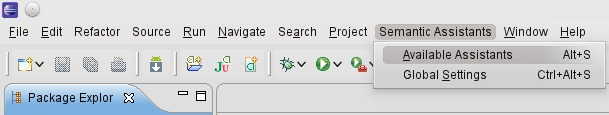
\includegraphics[width=1.0\textwidth]{pictures/eclipse_menu.jpg}
  \caption{Semantic Assistant Menu in Eclipse}
  \label{fig:eclipse_menu}
\end{center}
\end{figure}
\subsection{Available Assistants}
Selecting the ``Available Assistants'' item from Semantic Assistants menu will
open a file selection dialog. The file selection dialog allows the user to
select the desired files, folders and even complete projects to send to the
server as inputs to an NLP service. For more convenience, you can type an arbitrary extension like ``java'' or ``xml'', in the ``File Format'' field to filter to file tree view. 

\begin{figure}[htb]
\begin{center}
  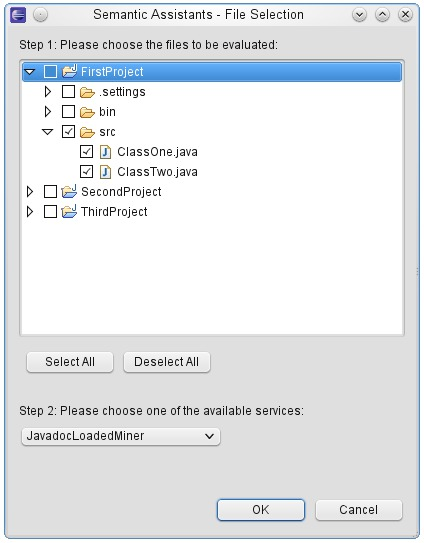
\includegraphics[width=0.5\textwidth]{pictures/eclipse_fileSelection.jpg}
  \caption{File Selection Dialog}
  \label{fig:eclipse_fileSelection}
\end{center}
\end{figure}

This dialog also lets the user to select an NLP service from a dynamically
generated list of services. This list is generated dynamically by selecting the
available services based on the client and the language capabilities of the
deployed NLP services. The server location where the service information are read from is presented just above the list as depicted in Fig \ref{fig:eclipse_services}. Note that the integration of a new service does not
require any changes on the client side - any new NLP service created and
deployed by a language engineer is dynamically discovered through its OWL
metadata maintained by the architecture and so becomes immediately available to
any connected client.

\begin{figure}[htb]
\begin{center}
  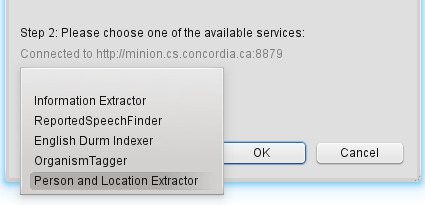
\includegraphics[width=0.5\textwidth]{pictures/eclipse_services.jpg}
  \caption{A List of Available NLP Services}
  \label{fig:eclipse_services}
\end{center}
\end{figure}

Upon selecting the resource files and the desired service, the user can execute
the selected service on the checked files in the tree. Consequently, the user will be informed about the status of the execution in the ``Semantic Assistant Status'' view. A successful execution of the selected NLP service, will let the user know on how to view the results. If the service execution fails, a description of the occurred error will be shown to the user and invocation will be aborted.

Now, let's look at how different types of outputs are handled in the plug-in:

\paragraph{Annotations.}
Annotations retrieved from a successful service invocation are being shown to the user in an
Eclipse view part called ``Semantic Assistants'' view. In the mentioned view, a
table will be dynamically generated that contains
all the parsed annotation instances. In Figure~\ref{fig:eclipse_saView} the
result of an execution of the ``Person and Location Extractor'' service on two
sample classes is shown.
\begin{figure}[htb]
\begin{center}
  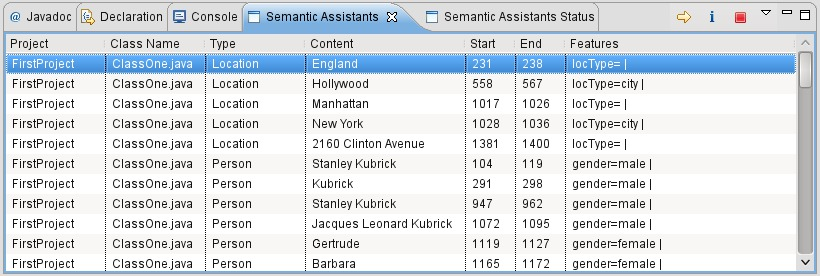
\includegraphics[width=1\textwidth]{pictures/eclipse_saView.jpg}
  \caption{Semantic Assistants View}
  \label{fig:eclipse_saView}
\end{center}
\end{figure}

This table can be sorted by different criteria through clicking on each column
title. Additionally, by double-clicking on each row in the table, the selected
annotation will appear with a graphical representation attached to the
corresponding resource. For instance, in Figure~\ref{fig:eclipse_annotation} the
JavadocMiner service has been invoked on a Java source code file. Some of the
annotations returned by the server bear a \emph{lineNumber} feature, which
attaches an annotation instance to a specific line in the java source file. Upon
double-clicking on the annotation instance in the Semantic Assistant view, the
corresponding resource - here, a .java file - will be opened in an editor and an
Eclipse warning marker will appear next to the line defined by the annotation
\emph{lineNumber} feature.

\begin{figure}[htb]
\begin{center}
  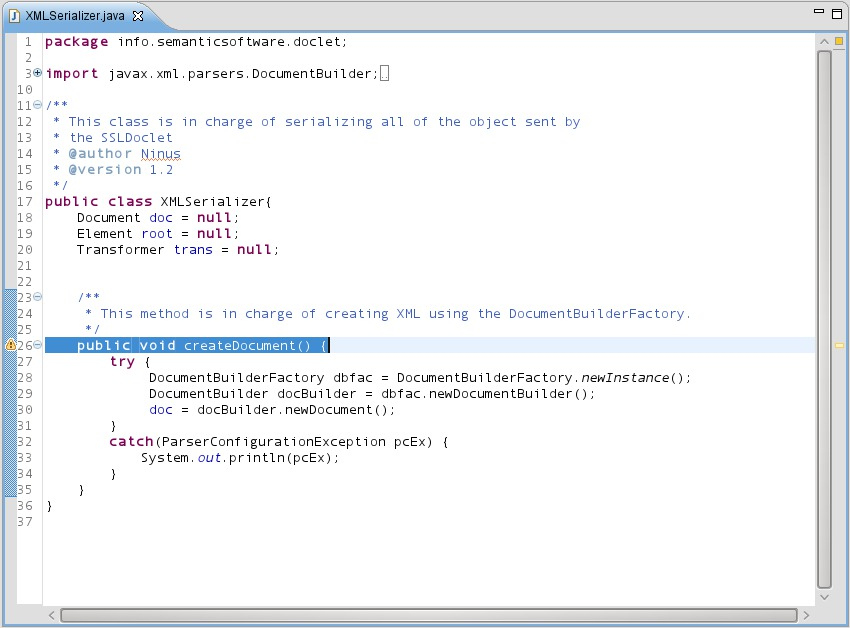
\includegraphics[width=1\textwidth]{pictures/eclipse_annotation.jpg}
  \caption{A Semantic Annotation}
  \label{fig:eclipse_annotation}
\end{center}
\end{figure}

\paragraph{Boundless Annotations.}
Boundless Annotations are a special kind of Annotations that adhere to a whole document and thus have no start and end offset. The plug-in parses the annotation results, and then inserts the content of the annotations in a new document and opens it in a new editor inside the Eclipse environment.

\paragraph{Documents.}
Documents received from the server response carry a URL property where defines where they are located. The plug-in retrieves the URLs and inserts them into a new document that opens up in a new editor inside the Eclipse environment.

\paragraph{Files.}
When a file output type is received by the plug-in, it will try to open it up in a web browser. In Eclipse, users can configure whether they want to open URLs in the Eclipse built-in web browser or any other ones in the file system. Whichever defined as the default behavior in Eclipse by the user, will be used by the plug-in to present the result file to the user. In this case, a log message will be shown to the user in the ``Semantic Assistants Status'' view to inform the user that the file is opened in his browser.

\subsection{Global Settings}
The second option found under the Semantic Assistants menu is the ``Global
Settings'' item. By clicking on this menu item, a dialog as depicted in Figure \ref{fig:eclipse_settings} is shown to the user that lets him choose a preferred server from a list of pre-defined values or add a custom server to the settings file. The values are provided in the Semantic Assistants global preference file described in \ref{sec:pref_management}. If the preference file gets accidentally deleted, a default preference file will be created by the plug-in but the eclipse-specific settings will be lost.
\begin{figure}[htb]
\begin{center}
  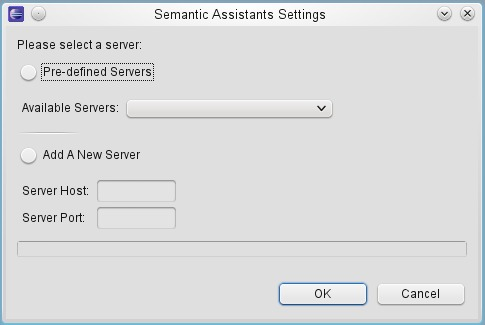
\includegraphics[width=0.6\textwidth]{pictures/eclipse_settings.jpg}
  \caption{Semantic Assistants Server Settings Dialog}
  \label{fig:eclipse_settings}
\end{center}
\end{figure}

\section{Installation}
\label{subsec:eclipse_install}
You can install the Semantic Assistants plug-in via the Eclipse software installer. To do so, first you have to add the Semantic Assistants software repository to your Eclipse list of software sites. In addition to installing the plug-in, adding the repository lets the Eclipse update manager to check for plug-in updates once available. Please carefully follow the steps listed below to install the Eclipse plug-in and refer to section \ref{trouble:eclipse_install} for installation troubleshooting.

\begin{enumerate}
  \item Select Help $\rightarrow$ Install New Software to open the Eclipse software installer.
  \item Press the ``Add'' button in the dialog, to add the Semantic Assistants repository.
  \item In the new dialog depicted in Fig \ref{fig:eclipse_install}, type ``\texttt{Semantic Assistants}'' and\\ ``\texttt{http://sa-eclipse.semanticsoftware.info}'' in ``Name'' and ``Location'' fields, respectively, and press ``OK''.
  \item The Semantic Assistants repository should now be added to your Eclipse list of software sites as seen in Fig \ref{fig:eclipse_install2}. From the loaded softwares, check the Eclipse plug-in and press ``Next''.
  \item Simply, follow the installation steps and let the installer restart the Eclipse application.
  \item The Eclipse plug-in loader will automatically load the plug-in for you. If the plug-in is installed
successfully, you should be able to see the Semantic Assistants menu added to
you toolbar.
\end{enumerate}

\begin{figure}[htb]
\begin{center}
  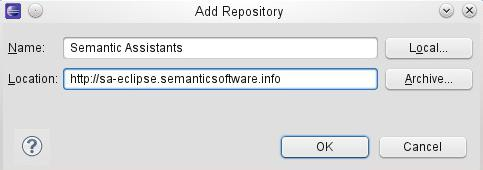
\includegraphics[width=0.6\textwidth]{pictures/eclipse_install.jpg}
  \caption{Adding Semantic Assistants Repository to Eclipse List of Software Sites}
  \label{fig:eclipse_install}
\end{center}
\end{figure}

\begin{figure}[htb]
\begin{center}
  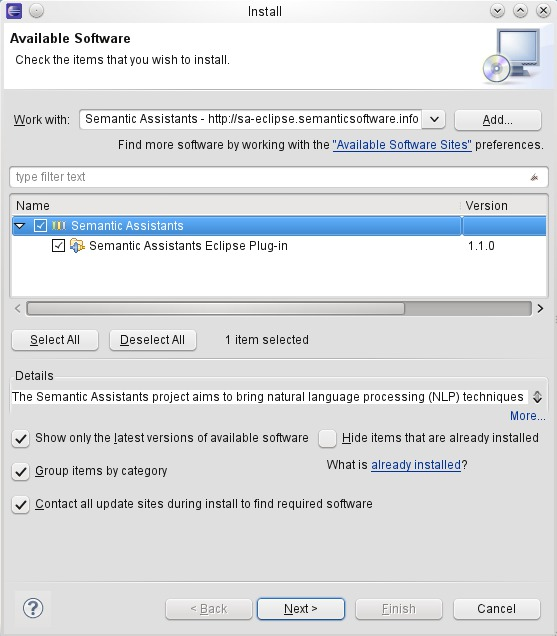
\includegraphics[width=0.6\textwidth]{pictures/eclipse_install2.jpg}
  \caption{Eclipse Software Installer Dialog}
  \label{fig:eclipse_install2}
\end{center}
\end{figure}

\section{Updating The Plug-in}
\begin{enumerate}
  \item Select Help $\rightarrow$ Check for Updates to open the Eclipse update manager.
  \item If there are any updates available for the Semantic Assistants plug-in, it will appear the in the update manager dialog as shown in Fig \ref{fig:eclipse_update}.
  \item Check the Semantic Assistants Eclipse plug-in from the list and press ``Next''.
  \item Follow the wizard steps and let the update manager restart your Eclipse for the updates to take place.
\end{enumerate}

\begin{figure}[htb]
\begin{center}
  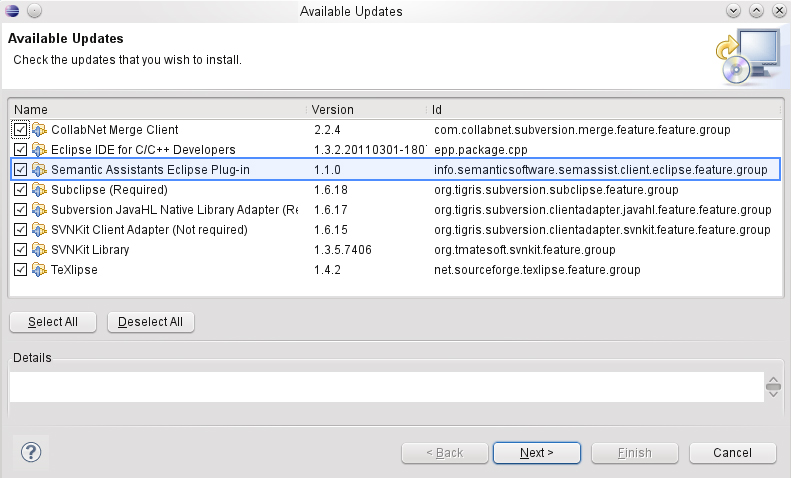
\includegraphics[width=1.0\textwidth]{pictures/eclipse_update.jpg}
  \caption{Updatin the Plug-in via Eclipse Update Manager}
  \label{fig:eclipse_update}
\end{center}
\end{figure}

\section{Development Notes}
\label{subsec:eclipse.development}
In this section, we provide further technical details on our plug-in for
developers interesting in enhancing or modifying it.

\subsection{Plug-in Source Directory Structure}
The Semantic Assistants plug-in uses Model-View-Controller pattern for its
implementation. Thus, most of the source code files are divided into different
packages related to their responsibilities. When you browse to
\url{src/info/semanticsoftware/semassist/client/eclipse/} folder, you see the
following structure:
\begin{enumerate}
\item\url{dialogs}: This folder contains the dialogs that are shown to the user
for interactions e.g. file selection. The classes inside this folder are the
codes for graphical user interfaces.
\item\url{handlers}: This folder contains the classes which play the controller
role in MVC pattern. Examples of these classes are dialog handlers and service
invocation jobs.
\item\url{model}: This folder contains the classes that provide data for
graphical user interfaces. These models are consumed by classes inside
\texttt{views} package.
\item\url{utils}: This folder contains utility classes e.g. logging feature.
\item\url{views}: This folder contains the source codes for Semantic Assistants
view parts. These are again graphical user interfaces but packaged differently
from dialogs.
\end{enumerate}

There is also another file called \url{Activator.java} in the source directory.
It is the main class of the plug-in that will be loaded initially and control
the plug-in's life cycle.

\subsection{Modifying the Plug-in}
If you want to modify the plug-in behavior or enhance it, follow these steps:
\begin{enumerate}
\item Open the Eclipse application.
\item Select File $\rightarrow$ New  $\rightarrow$ Project and under the
``Plug-in Development'' category select the ``Plug-in Project''.
\item A new plug-in project wizard will open up. Keep the EclipsePlugin name for
the project. Just below the project name there is a checkbox reading ``Use
Default Location''. Uncheck it and browse to the EclipsePlugin folder inside
where you've stored the Semantic Assistants folder.
\item Leave the other options untouched and press Finish.
\end{enumerate}

\begin{figure}[htb]
\begin{center}
  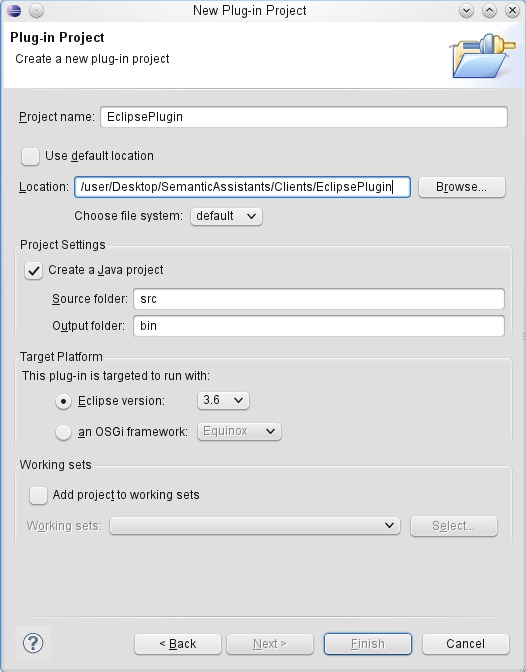
\includegraphics[width=0.5\textwidth]{pictures/eclipse_project_wizard.jpg}
  \caption{Eclipse New Plug-in Project Wizard}
  \label{fig:eclipse_project_wizard}
\end{center}
\end{figure}

\textbf{Note:} Remember you should manually copy the CSAL.jar file into you the
project's \texttt{lib} folder because it is a part of the project's dependency
and is defined in the classpath.

When the project is loaded in your workspace, feel free to play around. Browse
the source directory and add your development codes. To run your code, right
click on \texttt{plugin.xml} file and select Run As $\rightarrow$ Eclipse
Application.
